\chapter{Implementazione e manuale utente}

\begin{preamble}
{\em Questo capitolo assume una notevole importanza poiché tratterà diversi aspetti cruciali del progetto. Si inizierà esaminando la procedura per la creazione e l'importazione di nuovi oggetti tridimensionali all'interno dell'applicazione Unity. \newline \indent Successivamente, verrà affrontata l'implementazione in codice C\# delle classi descritte nel capitolo precedente. Inoltre, verrà fornita una descrizione dettagliata del processo di creazione delle animazioni utilizzate nel menù principale e nella scena dedicata alla selezione dell'annata del prodotto vitivinicolo.\newline \indent Infine, nell'ultima sezione, verrà presentato un manuale utente completo che guiderà gli utenti nell'utilizzo dell'applicazione in modo semplice ed efficace.}
\end{preamble}

\section{Creazione ed importazione di un modello tridimensionale di un prodotto}
\subsection{Creazione del modello tridimensionale dell'oggetto tramite smartphone}

In questa sezione verrà descritto il processo di creazione ed importazione di un modello tridimensionale di un prodotto vitivinicolo per consentire successivamente a Vuforia Engine di riconoscerlo tramite l'applicazione Android sviluppata in Unity.

Come precedentemente menzionato, il primo passo consiste nella generazione di un modello tridimensionale utilizzando l'applicazione mobile \textit{PolyCam}. Dopo aver creato un account gratuito tramite l'applicazione, è stata scelta la modalità \textit{Photo Mode} per scattare una serie di fotografie dell'oggetto da utilizzare per la costruzione del modello tridimensionale. Nel caso del progetto, per ottenere un risultato ottimale, sono state scattate oltre 100 fotografie della bottiglia di vino ed è stato necessario il posizionamento dell'oggetto all'interno di un set fotografico ben preparato, in quanto è importante eliminare qualsiasi "rumore" o "disturbo" presente nello sfondo. Infatti, è consigliato posizionare un pannello o un cartoncino scuro dietro all'oggetto per evitare che altri oggetti interferiscano con la costruzione del modello tridimensionale. Nel progetto, è stata utilizzata una scatola di cartone posta dietro alla bottiglia di vino della cantina Strappelli come mostrato in Figura \ref{5fig:setBottiglia}.

\begin{figure}[h]
	\centering
	\includegraphics [width=.50\columnwidth, angle=0]
            {setBottiglia}
	\caption{Il set utilizzato per creare il modello 3D}
	\label{5fig:setBottiglia}
\end{figure}

Inoltre, le foto devono essere scattate in modo tale da ottenere una panoramica completa a 360$^\circ$ della bottiglia. Per raggiungere questo obiettivo, essa è stata posizionata su una piattaforma girevole, consentendone, così, la rotazione durante l'acquisizione delle immagini in sequenza.

Una volta ottenute le immagini dell'oggetto, esse vengono inviate al server di PolyCam. In poco tempo, viene fornito un modello tridimensionale dell'oggetto desiderato nel formato glTF.

\subsection{Raffinamento del modello tridimensionale con Blender}

Il modello tridimensionale fornito da \textit{PolyCam} solitamente mostra delle imperfezioni dovute al rumore presente nelle immagini acquisite. Nel caso della bottiglia di vino, è stato necessario rimuovere, tramite l'utilizzo di Blender, alcune imperfezioni che si trovavano nella parte superiore e alla base dell'oggetto, poiché rappresentavano porzioni dello sfondo erroneamente incluse nel modello tridimensionale.
Di seguito sono riportati il modello prima (Figura \ref{5fig:preBlender}) e dopo (Figura \ref{5fig:postBlender}) le correzioni effettuate in Blender. 

\begin{figure}[h]
	\centering
	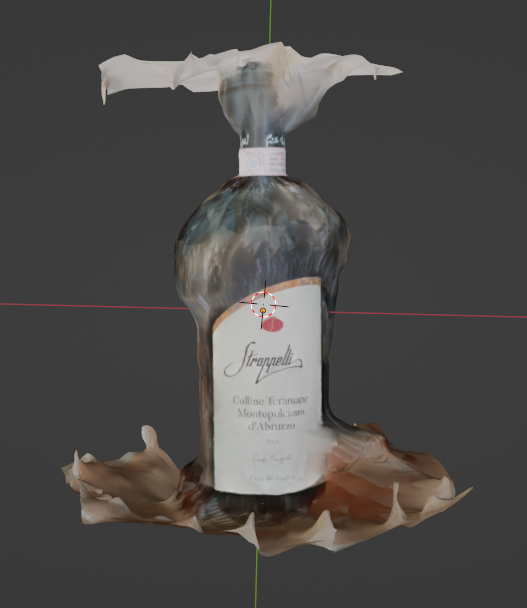
\includegraphics [width=.45\columnwidth, angle=0]
            {preBlender}
	\caption{Modello 3D prima dell'utilizzo di Blender}
	\label{5fig:preBlender}
\end{figure}

\begin{figure}[h]
	\centering
	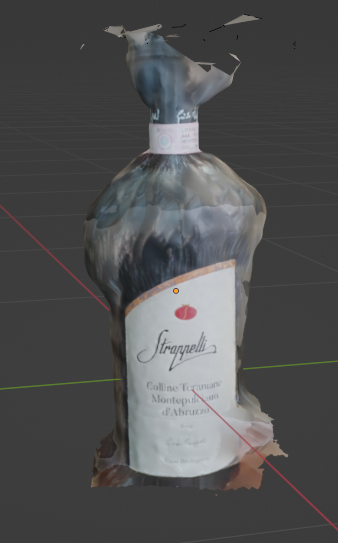
\includegraphics [width=.35\columnwidth, angle=0]
            {postBlender}
	\caption{Modello 3D dopo l'utilizzo di Blender}
	\label{5fig:postBlender}
\end{figure}

\subsection{Creazione ed importazione di un modello in Vuforia Engine}

Una volta corretto il modello con Blender, è possibile esportarlo nel formato glTF richiesto da Vuforia. Successivamente, è necessario creare un account e una licenza gratuita sul portale degli sviluppatori di Vuforia.

Una volta ottenuta la licenza, è necessario importare il file glTF precedentemente creato all'interno di \textit{Vuforia Model Target Generator}. Questo strumento rielaborerà il modello in modo tale da essere poi importato tramite il \textit{Package Manager} di Unity. Successivamente, si procede ad importare \textit{Vuforia Engine} tramite l'\textit{Asset Store} di Unity. Nella scena dedicata al riconoscimento delle bottiglie, è stato inserito un oggetto chiamato \textit{Model Target} che contiene gli strumenti del motore grafico Vuforia utili per eseguire il riconoscimento del prodotto vitivinicolo tra cui il modello tridimensionale creato in precedenza. L'oggetto \textit{Model Target} è mostrato in Figura \ref{5fig:modelTargetScene}. 

All'interno di quest'ultimo, si trova uno script C\# chiamato \textit{ObjectTrackingHandler} che include una classe omonima e un metodo specifico denominato \textit{OnTrackingFound}. Quest'ultimo consente, per prima cosa, di salvare il nome dell'oggetto riconosciuto in una variabile chiamata \textit{trackedObjectName} per poi, in secondo luogo, caricare la scena successiva dedicata alla selezione dell'annata di riferimento del vino.

\begin{figure}[h]
	\centering
	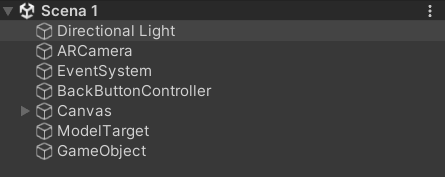
\includegraphics [width=.45\columnwidth, angle=0]
            {modelTargetScene}
	\caption{Posizionamento dell'oggetto \textit{ModelTarget} nella scena}
	\label{5fig:modelTargetScene}
\end{figure}

\section{Implementazione delle classi principali}

Nel capitolo precedente, sono stati forniti i Class Diagram delle classi più importanti che permettono di implementare le funzionalità principali dell'applicazione Android. In questa sezione, si mostrerà il codice per ognuna delle classi create.

\subsection{Implementazione della classe IotAPICaller}

Come già accennato in precedenza, la classe \textit{IotAPICaller} permette all'applicazione Android di ottenere i dati in tempo reale dalla stazione IoT presente nel vigneto di proprietà della cantina Strappelli. Nel Listato \ref{lst:IotAPICallerScript} è mostrato il codice della classe.

\begin{lstlisting}[caption=Codice sorgente dello script \textit{IotAPICaller}, label=lst:IotAPICallerScript, captionpos=b, basicstyle=\scriptsize]

using Newtonsoft.Json;
using System;
using System.Collections.Generic;
using System.Globalization;
using System.IO;
using System.Net;
using System.Text;
using System.Threading.Tasks;
using UnityEngine;
using UnityEngine.Networking;
using UnityEngine.UI;


public class IotAPICaller: MonoBehaviour
{
    public string status { get; set; }
    public List<string> head { get; set; }
    public List<List<string>> data { get; set; }
    public int rows { get; set; }

    

    [SerializeField] private Text txtLeafTemp;
    [SerializeField] private Text txtLeafHum;
    [SerializeField] private Text txtTemp;
    [SerializeField] private Text txtHum;
    [SerializeField] private Text txtRain;
    [SerializeField] private Text txtLatestUpd;
    void Start()
    {       
        HttpWebRequest request = (HttpWebRequest)WebRequest.Create("http://13.51.174.103:6041/rest/sql");
        request.ContentType = "application/json";
        request.Method = "POST";
        request.Headers.Add("Authorization", "Basic " + "cm9vdDp0YW9zZGF0YQ==");
        request.ContentType = "application/json";        
        
        Stream dataStream = request.GetRequestStream();
        string sql = "select * from station1.sensor_data where ts >= NOW - 48h order by ts DESC limit 1";
        byte[] byteArray = Encoding.ASCII.GetBytes(sql);
        dataStream.Write(byteArray, 0, byteArray.Length);
        HttpWebResponse response = (HttpWebResponse)request.GetResponse();
        string responseString = new StreamReader(response.GetResponseStream()).ReadToEnd();
        
        IotAPICaller apiData = JsonConvert.DeserializeObject<IotAPICaller>(responseString);
        
        txtLeafTemp.text = (apiData.data[0][11].ToString().Substring(0, 5) + " \si{\degreeC}C");
        txtLeafHum.text = (apiData.data[0][10].ToString().Substring(0, 3) + " %");
        txtTemp.text = (apiData.data[0][2].ToString().Substring(0, 5) + " \si{\degreeC}C");
        txtHum.text = (apiData.data[0][3].ToString().Substring(0, 5) + " %");
        txtRain.text = (apiData.data[0][4].ToString().Substring(0, 3) + "  mm");
        
        DateTime latestUpdDate = DateTime.ParseExact(apiData.data[0][1].ToString().Substring(0, 10), "yyyy-MM-dd" , CultureInfo.InvariantCulture);
        DateTime latestUpdTime = DateTime.ParseExact(apiData.data[0][1].ToString().Substring(11, 5), "HH:mm", CultureInfo.InvariantCulture);
        txtLatestUpd.text = (latestUpdDate.ToString("dd-MM-yyyy") + " " + latestUpdTime.AddHours(2).ToString("HH:mm"));
    }
    
    
    
    public void UpdateData()
    {
        txtLeafTemp.text = "";
        txtLeafHum.text = "";
        txtTemp.text = "";
        txtHum.text = "";
        txtRain.text = "";
        txtLatestUpd.text = "";
        
        Start();
    }
   
}

\end{lstlisting}

L'inizio dello script include una serie di dichiarazioni di namespace, che forniscono accesso a librerie di terze parti e funzionalità di base. Alcuni di questi namespace includono \textit{Newtonsoft.Json} per il parsing JSON, \textit{System} namespace principale di C\#, \textit{System.Collections.Generic} per liste generiche, \textit{System.Globalization} per il supporto multilingue, \textit{System.IO} per operazioni di I/O, \textit{System.Net} per comunicazione di rete, \textit{System.Text} per lavorare con stringhe e \textit{UnityEngine} per le funzionalità specifiche di Unity.

La classe \textit{IotAPICaller} è definita come una classe derivata da \textit{MonoBehaviour}, il che significa che è progettata per essere associata ad un oggetto  \textit{GameObject} in Unity. Questa classe ha diverse proprietà pubbliche, come \textit{status}, \textit{head}, \textit{data}, \textit{rows}, che rappresentano i dati ricevuti dall'API come già anticipato nel capitolo precedente.

La classe contiene campi serializzati (\textit{[SerializeField]}) che rappresentano oggetti di testo (di tipo \textit{Text}) nell'interfaccia utente Unity. Questi campi verranno popolati con dati ricevuti dall'API e utilizzati per visualizzare le informazioni sull'interfaccia utente.

Il metodo \textit{Start()} è un metodo speciale di Unity che viene chiamato quando il componente viene inizializzato. All'interno di questo metodo:

\begin{itemize}
	
	\item Viene creata una richiesta HTTP di tipo POST \textit{(HttpWebRequest)} per l'URL specificato \textit{(http://13.51.174.103:6041/rest/sql)}.
	\item Vengono impostati vari dettagli sulla richiesta, come il tipo di contenuto \textit{(application/json)}, il metodo \textit{(POST)}, e l'autorizzazione (tramite un'intestazione \textit{Authorization}) per poter accedere ai dati presenti nella piattaforma cloud della stazione IoT.
	\item Viene creato un flusso di dati (\textit{dataStream}) per l'invio di essi nella richiesta, e viene inviata una query SQL al server IoT. Quest'ultima richiede tutti i campi della tabella \textit{station1.sensor\_data} in una finestra temporale di 48 ore prendendo soltanto il primo record che corrisponde al dato più recente grazie al comando di ordinamento decrescente eseguito sul campo timestamp \textit{ts}.
	\item Viene ricevuta una risposta \textit{HTTP} dal server IoT e il suo contenuto viene letto e memorizzato come una stringa.
	\item La stringa di risposta JSON viene deserializzata utilizzando \textit{JsonConvert} in un oggetto \textit{IotAPICaller}. I dati ricevuti vengono estratti e utilizzati per aggiornare i campi di testo nell'interfaccia utente Unity.
	\item Il metodo \textit{UpdateData()} cancella il contenuto dei campi di testo e, quindi, richiama il metodo \textit{Start()} per effettuare una nuova richiesta e aggiornare i dati.
\end{itemize}

\subsection{Implementazione della classe OpenWeatherAPICaller}

La seconda classe implementata nel progetto, chiamata \textit{OpenWeatherAPICaller}, si occupa di richiamare i dati provenienti dall'API di OpenWeather, come già descritto nel capitolo precedente. Nel Listato \ref{lst:OpenWeatherAPICallerScript} è presente l'implementazione in C\# della classe.

\begin{lstlisting}[caption=Codice sorgente dello script \textit{OpenWeatherAPICaller}, label=lst:OpenWeatherAPICallerScript, captionpos=b, basicstyle=\scriptsize]

using System;
using System.Collections;
using System.Collections.Generic;
using System.Threading.Tasks;
using UnityEngine;
using UnityEngine.Networking;
using UnityEngine.UI;

// Define a class structure to match the JSON data
[System.Serializable]
public class Coord
{
    public float lon;
    public float lat;
}

[System.Serializable]
public class Weather
{
    public int id;
    public string main;
    public string description;
    public string icon;
}

[System.Serializable]
public class Main
{
    public float temp;
    public float feels_like;
    public float temp_min;
    public float temp_max;
    public int pressure;
    public int humidity;
    public int sea_level;
    public int grnd_level;
}

[System.Serializable]
public class Wind
{
    public float speed;
    public int deg;
    public float gust;
}

[System.Serializable]
public class Clouds
{
    public int all;
}

[System.Serializable]
public class Sys
{
    public int type;
    public int id;
    public string country;
    public int sunrise;
    public int sunset;
}

[System.Serializable]
public class WeatherData
{
    public Coord coord;
    public Weather[] weather;
    public string baseData;
    public Main main;
    public int visibility;
    public Wind wind;
    public Clouds clouds;
    public int dt;
    public Sys sys;
    public int timezone;
    public int id;
    public string name;
    public int cod;
}

public class OpenWeatherAPICaller : MonoBehaviour
{
    private string openWeatherApiKey = "ea5f560544db2e6226f8c5da0c559f61";

    private float longitude = 0f;
    private float latitude = 0f;
    
    public MongoDBConnector mongoDBConnector;

    [SerializeField] private Image image;
    [SerializeField] private Text txtHealthDescription;
    [SerializeField] private Text txtLatestUpd;
    
    // Start is called before the first frame update
    async void Start()
    {
        if (longitude == 0f || latitude == 0f)
        {
            mongoDBConnector.GetDataAsync((data) =>
            {
                if (data != null)
                {
                    latitude = data.document.Latitudine;
                    longitude = data.document.Longitudine;
                }
            }, "lat_long");
        }
        
        await GetWeaherData();
    }
    
    private async Task GetWeaherData()
    {
        string url = $"https://api.openweathermap.org/data/2.5/weather?lat={latitude}&lon={longitude}&appid={openWeatherApiKey}&units=metric";

        using (UnityWebRequest webRequest = UnityWebRequest.Get(url))
        {
            var asyncOperation = webRequest.SendWebRequest();
            
            while (!asyncOperation.isDone)
            {
                await Task.Yield();
            }

            if (webRequest.result == UnityWebRequest.Result.ConnectionError || webRequest.result == UnityWebRequest.Result.ProtocolError)
            {
                Debug.LogError("Errore nella richiesta: " + webRequest.error);
                txtLatestUpd.text = "";
            }
            else
            {
                string json = webRequest.downloadHandler.text;
               
                WeatherData openWeatherData = JsonUtility.FromJson<WeatherData>(json);

                DateTime dateTime = UnixTimeStampToDateTime(openWeatherData.dt);
                
                string formattedDate = dateTime.ToString("dd/MM/yyyy HH:mm:ss", new System.Globalization.CultureInfo("it-IT"));

                txtLatestUpd.text = formattedDate;
                
                // temporale
                
                if ((openWeatherData.weather[0].id > 201 && openWeatherData.weather[0].id < 233))
                {
                    image.sprite = Resources.Load<Sprite>("Images/attention");
                    txtHealthDescription.text = "Oggi è una giornata difficile per il vigneto. C'e' un temporale in corso";
                    if (openWeatherData.wind.speed > 6f)
                    {
                        txtHealthDescription.text = "Oggi è una giornata difficile per il vigneto. C'e' un temporale in corso con forte vento";
                    }
                }
                else if ((openWeatherData.weather[0].id > 310 && openWeatherData.weather[0].id < 322) ||
                            (openWeatherData.weather[0].id > 502 && openWeatherData.weather[0].id < 533))
                {
                    image.sprite = Resources.Load<Sprite>("Images/attention");
                    txtHealthDescription.text = "Oggi nel vigneto sta piovendo molto... Potrebbe aumentare il rischio di malattie nel vigneto";
                    if (openWeatherData.wind.speed > 6f)
                    {
                        txtHealthDescription.text = "Oggi è una giornata difficile per il vigneto...Sta piovendo molto e tira un forte vento. Potrebbe aumentare il rischio di malattie nel vigneto";
                    }
                }else if ((openWeatherData.weather[0].id >= 600 && openWeatherData.weather[0].id < 623))
                {
                    image.sprite = Resources.Load<Sprite>("Images/attention");
                    txtHealthDescription.text = "Oggi nel vigneto sta nevicando! Potrebbe aumentare il rischio di malattie nel vigneto";
                    if (openWeatherData.wind.speed > 6f)
                    {
                        txtHealthDescription.text = "Oggi nel vigneto sta nevicando e tira un forte vento! Potrebbe aumentare il rischio di malattie nel vigneto";
                    }
                }else if ((openWeatherData.weather[0].id > 800 && openWeatherData.weather[0].id < 805))
                {
                    image.sprite = Resources.Load<Sprite>("Images/ok");
                    txtHealthDescription.text = "Oggi va tutto bene, ci sono soltanto delle nuvole...";
                    if (openWeatherData.wind.speed > 6f)
                    {
                        txtHealthDescription.text = "Oggi nel vigneto tira un forte vento! Potrebbe danneggiare il vigneto...";
                    }
                }else if (openWeatherData.weather[0].id == 800)
                {
                    image.sprite = Resources.Load<Sprite>("Images/ok");
                    txtHealthDescription.text = "Oggi va tutto bene nel vigneto!";
                }
                else
                {
                    image.sprite = Resources.Load<Sprite>("Images/ok");
                    txtHealthDescription.text = "Oggi va tutto bene nel vigneto!";
                }
                
                
            }
        }
        
    }
    
    public async void UpdateOpenWeatherData()
    {
        image.sprite = Resources.Load<Sprite>("Images/loading");
        
        txtHealthDescription.text = "";
        txtLatestUpd.text = "";
        
        await GetWeaherData();
    }
    
    // Function to convert Unix timestamp to DateTime
    private DateTime UnixTimeStampToDateTime(long unixTimestamp)
    {
        DateTime dateTime = new DateTime(1970, 1, 1, 0, 0, 0, DateTimeKind.Utc);
        dateTime = dateTime.AddSeconds(unixTimestamp).ToLocalTime();
        return dateTime;
    }
}


\end{lstlisting}

Di seguito verrà descritto il codice dettagliatamente:

\begin{itemize}
	\item La prima parte si occupa dell'importazione delle librerie:
	\begin{itemize}
		\item \textit{System}, \textit{System.Collections}, e \textit{System.Collections.Generic}, che rappresentano gli spazi dei nomi standard di C\#.
   		\item \textit{System.Threading.Tasks}, utilizzata per gestire operazioni asincrone.
   		\item \textit{UnityEngine}, che rappresenta il namespace di Unity.
   		\item \textit{UnityEngine.Networking}, utilizzata per eseguire richieste web.
   		\item \textit{UnityEngine.UI}, utilizzata per manipolare gli elementi dell'interfaccia utente nell'ambiente Unity.
	\end{itemize}
	\item La seconda parte del codice è dedicata alla definizione di classi utili per la deserializzazione dei dati provenienti dall'API \textit{OpenWeather}; le classi \textit{Coord}, \textit{Weather}, \textit{Main}, \textit{Wind}, \textit{Clouds}, \textit{Sys}, e \textit{WeatherData} sono utilizzate per corrispondere ai dati JSON restituiti dall'API di OpenWeatherMap. Queste classi sono annotate con \textit{[System.Serializable]} per consentire la serializzazione/deserializzazione dei dati JSON.
	\item Successivamente, il codice descrive le variabili di classe tra cui:
	\begin{itemize}
		\item \textit{openWeatherApiKey}, che contiene la chiave API per \textit{OpenWeather}.
   		\item \textit{longitude} e \textit{latitude}, che contengono le coordinate iniziali, inizializzate a 0.
   		\item \textit{mongoDBConnector}, che contiene un riferimento a un'istanza di un'altra classe per la connessione al database MongoDB.
   		\item \textit{image}, \textit{txtHealthDescription}, e \textit{txtLatestUpd}, che rappresentano riferimenti agli oggetti UI nell'interfaccia Unity.
	\end{itemize}
	\item Il metodo \textit{Start()} viene chiamato all'avvio dello script Unity e verifica se \textit{longitude} e \textit{latitude} sono uguali a 0. Se lo sono, cerca di ottenere queste coordinate dal database MongoDB utilizzando \textit{mongoDBConnector.GetDataAsync()}. Quindi, richiama il metodo \textit{GetWeatherData()} in modo asincrono.
\item Il metodo \textit{GetWeatherData()}:
	\begin{itemize}
		\item Costruisce l'URL per la richiesta API \textit{OpenWeather }utilizzando \textit{latitude}, \textit{longitude} e \textit{openWeatherApiKey}, che rappresenta la chiave di licenza.
		\item Invia una richiesta web asincrona utilizzando \textit{UnityWebRequest}.
		\item Attende il completamento della richiesta con un ciclo while.
		\item Se la richiesta è stata eseguita con successo, converte il risultato JSON in un oggetto della classe \textit{WeatherData}.
		\item Estrae i dati desiderati dall'oggetto \textit{WeatherData} e aggiorna l'interfaccia utente. Per individuare lo stato di salute del vigneto, si utilizzano il codice relativo alle condizioni meteo utilizzato da OpenWeather e la velocità del vento.
	\end{itemize}
\item Il metodo \textit{UpdateOpenWeatherData()}:
	\begin{itemize}
		\item viene chiamato quando si desidera aggiornare i dati meteorologici.
		\item mostra un'immagine di caricamento e cancella il testo nell'interfaccia utente.
		\item chiama il metodo \textit{GetWeatherData()} in modo asincrono per aggiornare i dati presenti nella UI di Unity.
	\end{itemize}
\item Il metodo \textit{UnixTimeStampToDateTime()} converte un timestamp UNIX in un oggetto \textit{DateTime} localizzato.
\end{itemize}

\subsection{Implementazione della classe ScriptManager}

L'obiettivo principale di questa classe è quello di visualizzare, scorrere ed evidenziare il testo dello script del sommelier in base al tempo corrente di esecuzione della traccia audio della recensione del vino. Nel Listato \ref{lst:ScriptManagerScript} è mostrato il codice della classe.

\begin{lstlisting}[caption=Codice sorgente dello script \textit{ScriptManager}, label=lst:ScriptManagerScript, captionpos=b, basicstyle=\scriptsize]

using System.Collections;
using System.Collections.Generic;
using UnityEngine;
using System;
using System.Linq;
using System.IO;
using UnityEngine.UI;
using System.Globalization;
using UnityEngine.EventSystems;

public class ScriptManager : MonoBehaviour
{
    public GameObject SoundManager;
    private string currentTime = "";
    private string[] splitDuration;
    List<string> scriptRedListed = new List<string>();
    List<string> scriptBlackListed = new List<string>();
    
    private Dictionary<int, string> scriptDict = new Dictionary<int, string>();
    private List<String> scriptList = new List<string>();

    [SerializeField] ScrollRect autoScrollRect;
    [SerializeField] private RectTransform contentRectTransform;
    [SerializeField] Text txtReview;
    public MongoDBConnector mongoDBConnector;
    
    // Start is called before the first frame update
    void Start()
    {
        
        mongoDBConnector.GetDataAsync((data) =>
        {
            if (data != null)
            {
                Dictionary<string, string> scriptSommelierSelected = data.document.ScriptSommelier[Scene2Setter.GetSelectedOption()];
                
                foreach (var kvp in scriptSommelierSelected)
                {
                    scriptDict[int.Parse(kvp.Key)] = kvp.Value; // Add the entry to the dictionary
                    
                }
                
            }
            else
            {
                Debug.LogError("Impossibile connettersi al DB!");
            }

            
        }, "script");
        
        foreach (KeyValuePair<int, string> scriptScorePair in scriptDict)
        {
            scriptList.Add(scriptScorePair.Value);
        }
        
        txtReview.text = (string.Join("\n", scriptList));

        if (autoScrollRect == null) autoScrollRect = GetComponent<ScrollRect>();

    }



// Update is called once per frame
    void Update()
    {
        currentTime = SoundManager.GetComponent<SoundManager>().getCurrentTime();

        int script_minutes = 0;
        int script_seconds = 0;

        splitDuration = currentTime.Split(':');

        if (splitDuration.Length > 1)
        {
            if (!(String.IsNullOrEmpty(splitDuration[0])) || !(String.IsNullOrEmpty(splitDuration[1])))
            {
                script_minutes = Int32.Parse(splitDuration[0]);
                script_seconds = Int32.Parse(splitDuration[1]);
            }
        }

        int totalSeconds = 0;

        totalSeconds = script_minutes * 60 + script_seconds;

        scriptRedListed = scriptDict
            .Where(item => item.Key <= totalSeconds)
            .Select(item => item.Value)
            .ToList();

        scriptBlackListed = scriptDict
            .Where(item => item.Key > totalSeconds)
            .Select(item => item.Value)
            .ToList();

        if (scriptRedListed.Count > 0)
        {
            scriptBlackListed.Insert(0, "");
        }

        txtReview.text = "<color=#8F1338>" + string.Join("\n", scriptRedListed) + "</color>" +
                         string.Join("\n", scriptBlackListed);

        // Calculate the total height of the content
        float totalContentHeight = contentRectTransform.rect.height;

        // Calculate the height of a single line of text in the ScrollView
        float lineHeight = txtReview.fontSize + txtReview.lineSpacing;

        float highlightedTextPosition = (scriptRedListed.Count * lineHeight);

        // Calculate the height of the ScrollView viewport
        float scrollViewViewportHeight = autoScrollRect.viewport.rect.height;

        // Calculate the maximum vertical scroll position (bottom-most position of the ScrollView)
        float maxVerticalScrollPosition = totalContentHeight - scrollViewViewportHeight;

        // Calculate the target vertical scroll position based on the highlighted text position
        float targetVerticalScrollPosition = Mathf.Clamp(highlightedTextPosition, 0f, maxVerticalScrollPosition);

        // Calculate the normalized vertical scroll position (between 0 and 1)
        float normalizedScrollPosition = targetVerticalScrollPosition / maxVerticalScrollPosition;

        if (normalizedScrollPosition < 0.058f)
        {
            autoScrollRect.verticalScrollbar.value = 1f;
            
        }else if(normalizedScrollPosition > 0.058f && normalizedScrollPosition < 0.32f)
        {
            autoScrollRect.verticalScrollbar.value = 1f - normalizedScrollPosition;
            
        }else if(normalizedScrollPosition > 0.32f && normalizedScrollPosition < 0.46f)
        {
            autoScrollRect.verticalScrollbar.value = 1f - normalizedScrollPosition - 0.1f;
        }
        else if (normalizedScrollPosition > 0.46f && normalizedScrollPosition < 0.53f)
        {
            autoScrollRect.verticalScrollbar.value = 1f - normalizedScrollPosition - 0.18f;
        }else
        {
            autoScrollRect.verticalScrollbar.value = 0f;
        }
        
    }

}

\end{lstlisting}

Di seguito verrà descritto il codice dettagliatamente:

\begin{itemize}
	\item La prima parte è dedicata all'importazione delle librerie necessarie per il progetto, come quelle dedicate alla gestione delle interfacce utente, del tempo e della connessione a un database MongoDB, e altro.
	\item La seconda parte si occupa di dichiarare le variabili che memorizzano i dati che verranno utilizzati nel codice, tra cui oggetti \textit{GameObject}, stringhe, liste e dizionari. Ad esempio, \textit{scriptRedListed} e \textit{scriptBlackListed} sono liste di stringhe, \textit{scriptDict} è un dizionario di interi e stringhe, \textit{autoScrollRect} è un riferimento a un oggetto \textit{ScrollRect} nell'interfaccia utente, e \textit{txtReview} è un riferimento a un oggetto di testo.
	\item La funzione \textit{Start()} viene chiamata quando il gioco inizia. Al suo interno, vengono eseguite le seguenti operazioni:
	\begin{itemize}
		\item Viene richiamata la funzione \textit{GetDataAsync} del componente \textit{mongoDBConnector} per ottenere dati da un database MongoDB.
		\item I dati ottenuti dal database vengono memorizzati in un dizionario chiamato \textit{scriptDict}.
		\item Viene creato un elenco \textit{scriptList} che contiene i valori del dizionario \textit{scriptDict}.
		\item Il testo visualizzato nell'oggetto \textit{txtReview} viene impostato utilizzando \textit{string.Join} per concatenare i valori dell'elenco \textit{scriptList}.
		\item Viene controllato se \textit{autoScrollRect} è nullo e, in caso affermativo, viene assegnato il componente \textit{ScrollRect} dell'oggetto corrente.
	\end{itemize}

\item Il metodo \textit{Update()} viene chiamato ad ogni frame e permette l'aggiornamento continuo della porzione di testo effettivamente letta dal sommelier nell'audio in esecuzione; esso si occupa anche di modificare lo scorrimento del componente \textit{ScrollRect} in base alla posizione in tempo reale dello script in riproduzione. In altre parole, l'obiettivo di questo metodo è garantire che il testo evidenziato sia sempre visibile all'utente durante la riproduzione dell'audio, garantendo un'esperienza simile al karaoke, dove il testo segue la traccia audio in tempo reale.

In particolare:
	\begin{itemize}
		\item La variabile \textit{currentTime} viene aggiornata con il tempo corrente dell'audio ottenuto da un oggetto chiamato \textit{SoundManager}. Il metodo \textit{getCurrentTime()} è utilizzato per recuperare il tempo corrente dell'audio in formato "minuti:secondi".
		\item Il tempo ottenuto viene suddiviso in minuti e secondi, e questi valori vengono memorizzati nelle variabili \textit{script\_minutes} e \textit{script\_seconds}.
		\item Il tempo totale dell'audio viene calcolato convertendo i minuti in secondi e sommandoli tra di loro. Questo valore viene memorizzato in \textit{totalSeconds}.
		\item L'elenco \textit{scriptRedListed} contiene il testo che deve essere visualizzato fino a quel momento nell'audio. Viene filtrato il dizionario \textit{scriptDict} in modo da includere solo le voci con un tempo chiave minore o uguale a \textit{totalSeconds}. Questo elenco conterrà il testo che deve essere visualizzato in evidenza.
		\item L'elenco \textit{scriptBlackListed} contiene il testo che non è ancora stato sincronizzato, ovvero il testo successivo a \textit{totalSeconds}. Viene filtrato il dizionario \textit{scriptDict} in modo da includere solo le voci con un tempo chiave maggiore di \textit{totalSeconds}.
		\item Il testo visualizzato nell'oggetto \textit{txtReview} viene aggiornato. Il testo evidenziato in \textit{scriptRedListed} viene reso rosso \textit{(<color=\#8F1338>)} mentre il testo non ancora sincronizzato in \textit{scriptBlackListed} rimane nel suo colore predefinito.
		\item Viene calcolata la posizione in pixel del testo evidenziato all'interno del \textit{txtReview}, tenendo conto dell'altezza del testo e del numero di righe evidenziate.
		\item Viene calcolata la posizione ideale per lo scorrimento verticale in base alla posizione del testo evidenziato rispetto alla vista dell'\textit{autoScrollRect}. Questo consente di posizionare la vista in modo che il testo evidenziato sia visibile all'utente.
		\item Sulla base della posizione calcolata, la barra di scorrimento verticale dell'\textit{autoScrollRect} viene regolata in modo che l'utente possa vedere il testo evidenziato senza doverlo scorrere manualmente.
	\end{itemize}
\end{itemize}


\subsection{Implementazione della classe MongoDBConnector}

Questa classe consente di effettuare richieste al servizio MongoDB e di ricevere dati in base a diversi tipi di query consentendo, così, di accedere a informazioni specifiche in base alle esigenze del gioco o dell'applicazione Unity. Nel Listato \ref{lst:MongoDBConnectorScript} è mostrato il codice della classe.

\begin{lstlisting}[caption=Codice sorgente dello script \textit{MongoDBConnector}, label=lst:MongoDBConnectorScript, captionpos=b, basicstyle=\scriptsize]

using UnityEngine;
using UnityEngine.Networking;
using System;
using System.Collections.Generic;
using Newtonsoft.Json;
using UnityEngine.UI;

[Serializable]
public class Document
{
    public string Titolo1;
    public string Titolo2;
    public float Latitudine;
    public float Longitudine;
    public Dictionary<string, string> Descrizione;
    public string LuogoProd;
    public Dictionary<string, Dictionary<string, string>> ScriptSommelier;
}

[Serializable]
public class JsonResponse
{
    public Document document;
}

public class MongoDBConnector : MonoBehaviour
{
    private const string apiKey = "lCcATJK57juG3SHbs16wDjaeniiK41kqdcQt51evKg4yGbGi0sVbegi47Lcw4MK1";
    private const string url = "https://us-east-1.aws.data.mongodb-api.com/app/data-wftpe/endpoint/data/v1/action/findOne";
    
    private string jsonData = "";
    
    private Action<JsonResponse> onDataReceived;

    public void GetDataAsync(Action<JsonResponse> callback, string queryType)
    {
        onDataReceived = callback;
        
        if (string.Compare(queryType, "all") == 0)
        {
            // Create a JSON object with your request data
            jsonData = "{\"collection\":\"Cantina\",\"database\":\"WineTech\",\"dataSource\":\"ClusterWineTech\",\"projection\":{},\"filter\":{\"Nome\":\"" + ObjectTrackingHandler.GetTrackedObjectName() + "\"}}";
            
        } else if (string.Compare(queryType, "lat_long") == 0)
        {
            jsonData = "{\"collection\":\"Cantina\",\"database\":\"WineTech\",\"dataSource\":\"ClusterWineTech\",\"projection\":{\"Latitudine\": 1, \"Longitudine\": 1},\"filter\":{\"Nome\":\"" + ObjectTrackingHandler.GetTrackedObjectName() + "\"}}";
            
        } else if (string.Compare(queryType, "tit1_tit2_luogo_descr") == 0)
        {
            jsonData = "{\"collection\":\"Cantina\",\"database\":\"WineTech\",\"dataSource\":\"ClusterWineTech\",\"projection\":{\"Titolo1\": 1, \"Titolo2\": 1, \"LuogoProd\": 1, \"Descrizione\": 1},\"filter\":{\"Nome\":\"" + ObjectTrackingHandler.GetTrackedObjectName() + "\"}}";
            
        }else if (string.Compare(queryType, "tit1_tit2_luogo") == 0)
        {
            jsonData = "{\"collection\":\"Cantina\",\"database\":\"WineTech\",\"dataSource\":\"ClusterWineTech\",\"projection\":{\"Titolo1\": 1, \"Titolo2\": 1, \"LuogoProd\": 1},\"filter\":{\"Nome\":\"" + ObjectTrackingHandler.GetTrackedObjectName() + "\"}}";
            
        }else if (string.Compare(queryType, "script") == 0)
        {
            jsonData = "{\"collection\":\"Cantina\",\"database\":\"WineTech\",\"dataSource\":\"ClusterWineTech\",\"projection\":{\"ScriptSommelier\": 1},\"filter\":{\"Nome\":\"" + ObjectTrackingHandler.GetTrackedObjectName() + "\"}}";
            
        }else if (string.Compare(queryType, "tit1_tit2_descr") == 0)
        {
            jsonData = "{\"collection\":\"Cantina\",\"database\":\"WineTech\",\"dataSource\":\"ClusterWineTech\",\"projection\":{\"Titolo1\": 1, \"Titolo2\": 1, \"Descrizione\": 1},\"filter\":{\"Nome\":\"" + ObjectTrackingHandler.GetTrackedObjectName() + "\"}}";
        }
        else
        {
            // Create a JSON object with your request data
            jsonData = "{\"collection\":\"Cantina\",\"database\":\"WineTech\",\"dataSource\":\"ClusterWineTech\",\"projection\":{},\"filter\":{\"Nome\":\"" + ObjectTrackingHandler.GetTrackedObjectName() + "\"}}";
        }
        
        // Create a UnityWebRequest
        UnityWebRequest request = new UnityWebRequest(url, "POST");
        request.SetRequestHeader("Content-Type", "application/json");
        request.SetRequestHeader("Access-Control-Request-Headers", "*");
        request.SetRequestHeader("api-key", apiKey);

        // Attach the request data
        byte[] bodyRaw = System.Text.Encoding.UTF8.GetBytes(jsonData);
        request.uploadHandler = (UploadHandler)new UploadHandlerRaw(bodyRaw);
        request.downloadHandler = (DownloadHandler)new DownloadHandlerBuffer();

        // Send the request asynchronously
        request.SendWebRequest().completed += (op) =>
        {
            // Handle the response when the request is complete
            if (request.result == UnityWebRequest.Result.Success)
            {
                // Parse the JSON response into a DocumentData object
           
                JsonResponse data = JsonConvert.DeserializeObject<JsonResponse>(request.downloadHandler.text);
                
                onDataReceived?.Invoke(data); // Invoke the callback with the data
                
            }
            else
            {
                Debug.LogError("Request failed: " + request.error);
                onDataReceived?.Invoke(null); // Invoke the callback with null to indicate an error
            }
        };
    }
}

\end{lstlisting}


Di seguito verrà descritto il codice dettagliatamente:

\begin{itemize}
	\item La prima parte è dedicata all'importazione delle librerie fondamentali per la classe come:
	\begin{itemize}
		\item \textit{UnityEngine} e \textit{UnityEngine.Networking}, che consentono di utilizzare le funzionalità di Unity per la gestione dell'ambiente di gioco e le richieste di rete.
		\item \textit{System.Collections.Generic}, che consente di utilizzare le collezioni di dati, come il dizionario.
		\item \textit{Newtonsoft.Json}, che consente la serializzazione e deserializzazione dei dati JSON.
		\item \textit{UnityEngine.UI}, che permette la gestione degli elementi dell'interfaccia grafica all'interno di Unity.
	\end{itemize}
	
	\item La seconda parte è dedicata alla definizione della classi utili per la deserializzazione dei dati provenienti dal documento MongoDB, ovvero:
	\begin{itemize}
		\item La classe \textit{Document} contiene vari campi, come \textit{Titolo1}, \textit{Titolo2}, \textit{Latitudine}, \textit{Longitudine}, \textit{Descrizione}, \textit{LuogoProd} e \textit{ScriptSommelier}, ognuno dei quali è associato a un tipo di dato specifico appartenente al documento MongoDB.
		\item La classe \textit{JsonResponse} rappresenta la struttura dei dati JSON restituiti dalla richiesta al servizio MongoDB. Essa contiene un campo \textit{document} che è un oggetto di tipo \textit{Document}.
	\end{itemize}
	\item La terza parte del codice è dedicata alla dichiarazione degli attributi tra cui:
	\begin{itemize}
		\item \textit{apiKey}: contiene l'API key del servizio MongoDB a cui si sta cercando di accedere.
		\item \textit{url}: è una stringa che contiene l'URL del servizio MongoDB a cui si sta cercando di accedere.
		\item \textit{jsonData}: è una variabile stringa che conterrà i dati JSON della richiesta.
		\item \textit{onDataReceived} è una variabile di tipo \textit{Action<JsonResponse>} che verrà utilizzata per passare una funzione di callback per elaborare i dati ricevuti.
	\end{itemize}
	\item L'ultima parte del codice definisce il metodo \textit{GetDataAsync} che viene utilizzato per effettuare una richiesta asincrona al servizio MongoDB.
Esso riceve due parametri ovvero \textit{callback} (la funzione di callback) e \textit{queryType} (il tipo di query da eseguire).
In base al valore di \textit{queryType}, viene costruita una stringa JSON (\textit{jsonData}) che rappresenta la richiesta da inviare al servizio MongoDB.
Viene creato un oggetto \textit{UnityWebRequest} per gestire la richiesta HTTP POST. Vengono impostati gli header e il corpo della richiesta.
La richiesta viene inviata in modo asincrono e un callback gestisce la risposta.
Se la richiesta ha successo, i dati JSON ricevuti vengono deserializzati in un oggetto \textit{JsonResponse} e passati alla funzione di callback \textit{onDataReceived}.
In caso di errore, viene generato un messaggio e la funzione di callback viene chiamata con \textit{null} per indicare un errore.
	
\end{itemize}

\section{Implementazione delle animazioni in Unity}

In questa sezione verranno riportate le implementazioni delle due animazioni principali presenti nell'applicazione Android. In particolare verranno descritte quelle presenti nel menù principale e nella pagina dedicata alla selezione dell'annata.

\subsection{Menù principale}

Il menù principale, come ampiamente descritto nel capitolo precedente, presenta un'animazione che fornisce i primi pulsanti dedicati alla selezione, rispettivamente, delle tre sezioni "Osserva", "Ascolta" e "Racconta". In Figura \ref{5fig:animazioneIntro} è mostrata la sequenza di operazioni compiute dall'animazione \textit{MenuFadeIn} all'avvio dell'applicazione.

\begin{figure}[h]
	\centering
	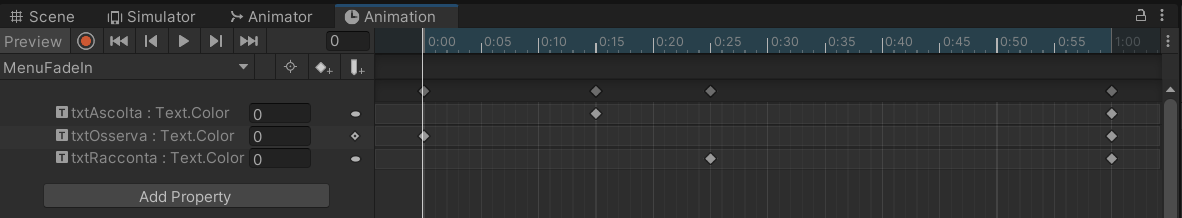
\includegraphics [width=.99\columnwidth, angle=0]
            {animazioneIntro}
	\caption{Sequenza di operazioni svolte all'avvio dell'applicazione dall'animazione \textit{MenuFadeIn}}
	\label{5fig:animazioneIntro}
\end{figure}

L'animazione è molto semplice: nel momento in cui l'applicazione è avviata, attiva un \textit{fadeIn} dei tre pulsanti "Osserva", "Ascolta" e "Racconta". Per creare l'effetto di dissolvenza in ingresso, viene modificata la componente \textit{alpha} del colore del testo dei pulsanti \textit{txtOsserva}, \textit{txtAscolta} e \textit{txtRacconta} portandolo da un valore iniziale di 0 fino ad 1. Ogni transizione ha un differente punto di partenza per creare un effetto gradevole all'utente.

In Figura \ref{5fig:animazioneSceltaOsserva} è fornita un'immagine della sequenza di operazioni che viene svolta nel momento in cui viene premuto il pulsante "Osserva". Per gli altri due pulsanti (Racconta e Ascolta), la sequenza di operazioni svolte dall'animazione è molto simile a quella descritta in seguito e quindi non verranno descritte.

\begin{figure}[h]
	\centering
	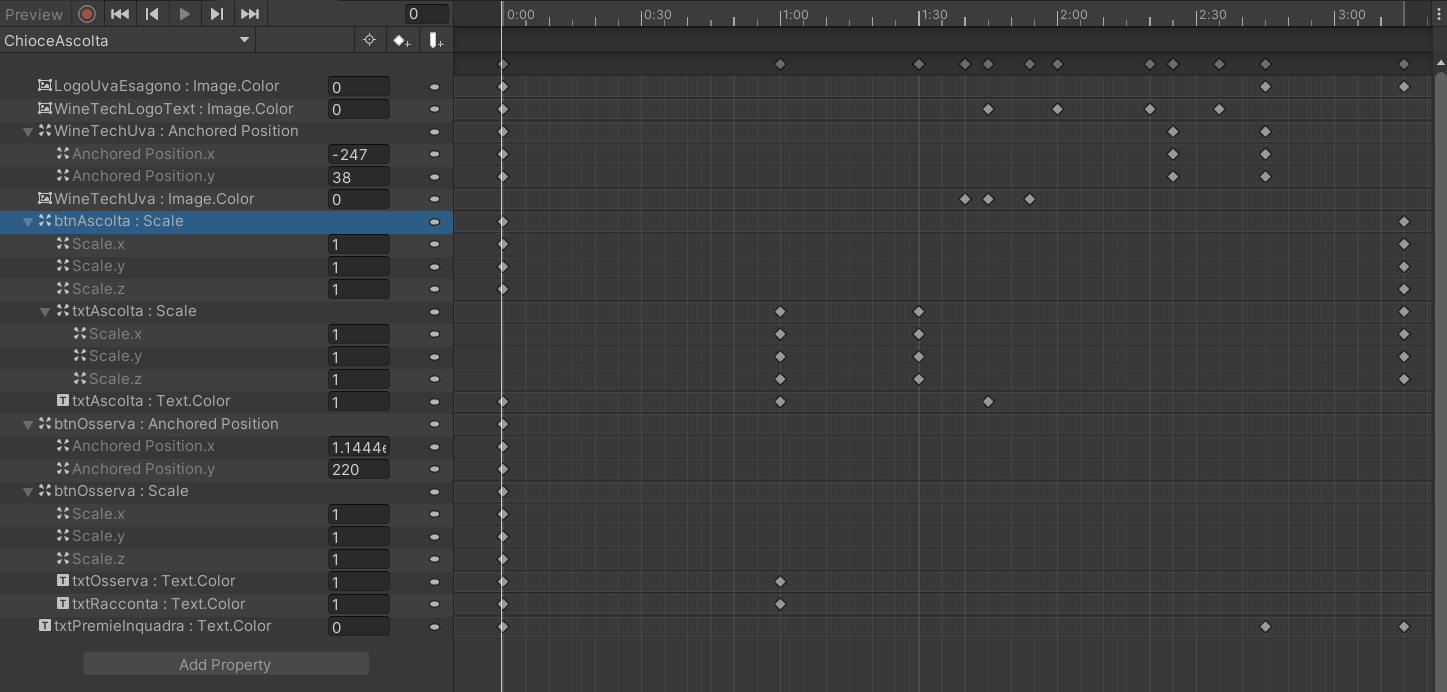
\includegraphics [width=.99\columnwidth, angle=0]
            {animazioneSceltaOsserva}
	\caption{Sequenza di operazioni svolte dall'animazione \textit{ChoiceOsserva}}
	\label{5fig:animazioneSceltaOsserva}
\end{figure}

Per prima cosa, nel momento in cui l'utente preme il pulsante "Osserva", viene effettuato un effetto di \textit{fadeOut} dei due pulsanti "Ascolta" e "Racconta", portando il valore di \textit{alpha} da 1 a 0 in maniera graduale. 

Subito dopo, viene effettuata una traslazione del pulsante "Osserva" dall'alto verso il centro modificando il parametro \textit{Anchored Position.y} dal valore 220 a 68 in maniera progressiva. 

Successivamente viene aumentata gradualmente la grandezza del pulsante portando i valori di \textit{Scale.x}, \textit{Scale.y} e \textit{Scale.z} da 1 ad 1.2, sempre in maniera graduale. Nel frattempo, viene inizializzata anche la transizione di \textit{fadeOut} del pulsante "Osserva" che porta il parametro \textit{alpha} del pulsante da 1 a 0. 

a questo punto vengono mostrate in modo temporalmente sfalsato, con un effetto \textit{fadeIn}, il logo dell'applicazione e la scritta "WineTech" (rispettivamente chiamati \textit{WineTechUva} e \textit{WineTechLogoText}), modificandone il parametro \textit{alpha} da 0 a 1 . 

Dopo appena un secondo, viene attivato il \textit{fadeOut} del pulsante \textit{WineTechLogoText} modificando il parametro \textit{alpha} da 1 a 0. Contemporaneamente viene effettuata una traslazione verso destra del logo dell'applicazione modificando il valore \textit{Anchored Position.x} da -245.19 a 2. Quasi in contemporanea, viene effettuato un \textit{fadeIn} del pulsante a forma di esagono che permette la transizione alla scena successiva, sempre modificando il parametro \textit{alpha} da 0 a 1 in maniera graduale.

\subsection{Selezione dell'annata}

Per quanto riguarda la schermata che permette la selezione dell'annata, l'animazione è più semplice rispetto a quella del menù principale. Infatti l'animazione coinvolta, denominata \textit{Scene2Intro}, effettua una modifica del parametro \textit{Anchored Position.y} dal valore -1080 a 0 per permettere lo scorrimento dal basso verso l'alto del pannello di selezione dell'annata. Successivamente, nel momento in cui la selezione è stata effettuata, viene ulteriormente incrementato il valore di \textit{Anchored Position.y} portandolo al valore di 0, ma stavolta del componente \textit{Background} dell'interfaccia grafica della scena.

\section{Manuale utente}

\subsection{Premessa}

Normalmente, un'applicazione Android è presente nel Google Play Store da cui è possibile scaricarla ed installarla in pochi minuti. Purtroppo quest'applicazione essendo un prototipo, non è ancora presente in questa piattaforma. Questa è la ragione per cui necessita di alcuni passaggi aggiuntivi per essere installata correttamente. In futuro, se il progetto verrà portato a compimento, l'applicazione sarà caricata all'interno del Google Play Store per essere aumentare l'accessibilità del prodotto. Tramite Unity, è possibile ottenere il file APK che consente l'installazione dell'applicazione una volta copiato il file all'interno dello smartphone. Bisogna, pertanto, avere l'autorizzazione da parte dell'utente per installare nuove applicazioni non certificate e quindi considerate pericolose.

\subsection{Effettuare il riconoscimento di un prodotto}

Una volta avviata l'applicazione, al primo utilizzo potrebbe essere richiesta l'autorizzazione per accedere alla fotocamera, che è essenziale per il riconoscimento dei prodotti vitivinicoli.

Dopo l'apertura dell'applicazione e l'apparizione dei pulsanti "Osserva," "Ascolta" e "Racconta" sullo schermo, è sufficiente premere il pulsante corrispondente alla sezione di interesse. Questa azione attiverà le animazioni e porterà alla visualizzazione del pulsante a forma di esagono. Quando si è in grado di avviare il riconoscimento del prodotto vitivinicolo, è possibile premere il pulsante per accedere alla schermata dedicata al riconoscimento.

L'operazione di riconoscimento avviene in modo automatico e se il prodotto viene identificato con successo, l'applicazione passerà alla schermata successiva che consente la selezione dell'annata del prodotto vitivinicolo. È sufficiente scegliere quest'ultima nel campo apposito e premere poi il pulsante "Avanti." A questo punto, l'utente sarà riportato alla schermata relativa alla scelta effettuata nelle prime fasi dell'applicazione.

\subsection{Utilizzo delle sezioni principali}

\subsubsection{Sezione Osserva}

La sezione \textit{Osserva} presenta una pagina singola con alcune informazioni sul prodotto vitivinicolo riconosciuto. L'utente può scorrere verso il basso per visualizzare il video dedicato all'azienda vitivinicola che viene riprodotto automaticamente.

\subsubsection{Sezione Ascolta}

Per quanto riguarda la sezione \textit{Ascolta}, basta attendere che il caricamento dello script sia effettuato da parte dell'applicazione. Una volta ottenuto il testo della recensione del sommelier, è sufficiente premere il pulsante \textit{Play} e, quindi, riprodurre l'audio relativo al prodotto vitivinicolo. Per tornare indietro o per andare avanti nella riproduzione, è sufficiente trascinare la barra di riproduzione verso destra o sinistra.

\subsubsection{Sezione Racconta}

La sezione \textit{Racconta}, invece, visualizza le informazioni in tempo reale associate al vigneto di provenienza del prodotto vitivinicolo. I dati vengono richiesti nel momento in cui viene attivata la sezione. Se si desidera aggiornare i dati relativi alla stazione IoT o quelli relativi a \textit{OpenWeather}, è possibile premere i relativi pulsanti presenti nell'interfaccia grafica.